
% ---------------------------------------------------------------------------------------------------------------
% It is an example which *does* use the .bib file (from which the .bbl file
% is produced).
% REMEMBER HOWEVER: After having produced the .bbl file,
% and prior to final submission,
% you need to 'insert'  your .bbl file into your source .tex file so as to provide
% ONE 'self-contained' source file.


\documentclass{acm_proc_article-sp}

\usepackage{algorithm}
\usepackage{algpseudocode}
%\usepackage{amsmath}

\newtheorem{theorem}{Theorem}
\newdef{definition}{Definition}

\begin{document}

\title{Gesture Recognition via 3D Accelerometer}


%
% You need the command \numberofauthors to handle the 'placement
% and alignment' of the authors beneath the title.
%
% For aesthetic reasons, we recommend 'three authors at a time'
% i.e. three 'name/affiliation blocks' be placed beneath the title.
%
% NOTE: You are NOT restricted in how many 'rows' of
% "name/affiliations" may appear. We just ask that you restrict
% the number of 'columns' to three.
%
% Because of the available 'opening page real-estate'
% we ask you to refrain from putting more than six authors
% (two rows with three columns) beneath the article title.
% More than six makes the first-page appear very cluttered indeed.
%
% Use the \alignauthor commands to handle the names
% and affiliations for an 'aesthetic maximum' of six authors.
% Add names, affiliations, addresses for
% the seventh etc. author(s) as the argument for the
% \additionalauthors command.
% These 'additional authors' will be output/set for you
% without further effort on your part as the last section in
% the body of your article BEFORE References or any Appendices.

\numberofauthors{3} %  in this sample file, there are a *total*
% of EIGHT authors. SIX appear on the 'first-page' (for formatting
% reasons) and the remaining two appear in the \additionalauthors section.
%
\author{
% You can go ahead and credit any number of authors here,
% e.g. one 'row of three' or two rows (consisting of one row of three
% and a second row of one, two or three).
%
% The command \alignauthor (no curly braces needed) should
% precede each author name, affiliation/snail-mail address and
% e-mail address. Additionally, tag each line of
% affiliation/address with \affaddr, and tag the
% e-mail address with \email.
%
% 1st. author
\alignauthor
Huihuang Zheng\\
       \affaddr{University of Texas at Austin}\\
       \email{huihuang@utexas.com}
% 2nd. author
\alignauthor
Yiming Pang\\
       \affaddr{University of Texas at Austin}\\
       \email{TODO}
}


\maketitle
\begin{abstract}
//TODO add this.
\end{abstract}


\category{Wireless Network}{Research Project}[report]

\terms{Algorithm, Application}

\keywords{Gesture, Accelerometer, Dynamic Time Warping(DTW)} % NOT required for Proceedings

\section{Introduction}
Gesture-based interactions are now widely used in mobile phone and laptop, which requires gesture pattern recognition. There are several methods to recognize gestures, for example, XBOX can recognize by vision approaching. Some researchers used wearable sensors like "glove" to detect motion of hands. But those works cost computing resource, power and hardware a lot. We focused on light-weight gesture recognition system: just use simple 3D accelerometer, which is common in your mobile phone.

Our project is mainly based on previous work uWave\cite{liu2009uwave}: A state of art gesture recognition method. It just uses templates of gesture. When it tries to detect gesture, it records gesture and uses Dynamic time warping(DTW) to compute time series Euclidean distance between gesture and templates. Then it outputs the template which matches best as recognition result. So it doesn't need a lot of computation or training compared to statistical methods.

What we have done are 1, Building the uWave on a Android mobile phone and run some experiments. 2, via experiment we got some shortcomings of uWave and we believe we could improve it. Our goal of this project is improving performance of gesture recognition and building an application based on gesture recognition. So we researched in advantages and disadvantages of uWave and then we make plan of our work.

Our report is organized as following: section 2 discussed the work of uWave. section 3 will show project and experiments we have done. We will show some shortcomings and what we can improve in the section. Section 4 shows our future plan, what we will add in our research project.

\section{uWave}
TODO write these or copy from paper\\
For recognition, uWave leverages a template library that stores one or more time series of known identities for every vocabulary gesture, often input by the user. Figure \ref{uWaveBasic} illustrates the recognition process. The input to uWave is a time series of
acceleration provided by a three-axis accelerometer. Each time sample is a vector of three elements, corresponding to the acceleration along the three axes. uWave first quantizes acceleration data into a time series of discrete values. The same quantization applies to the templates too. It then employs DTW to match the input time series against the templates of the gesture vocabulary. It recognizes the gesture as the template that provides the best matching. The recognition results,
confirmed by the user as correct or incorrect, can be used to adapt the existing templates to accommodate gesture variations over time.
\begin{figure}
  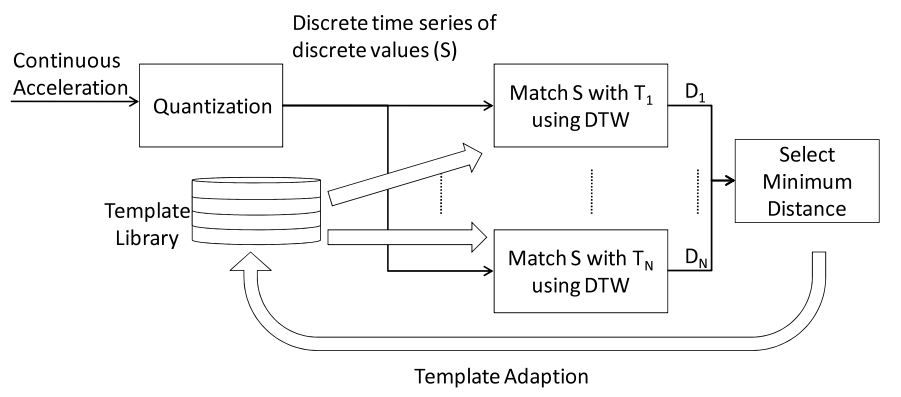
\includegraphics[width=0.8\linewidth]{uWave_basic.JPG}
  \caption{Basic idea of uWave}
  \label{uWaveBasic}
\end{figure}


\section{Project and Experiments We Have Done}
We implemented uWave on Android mobile phone and did some experiments about the recognition accuracy:  


\section{Future Plan}
We plan to do two aspects in the future, one is improving performance by SVM approaching. Another is implementing an application to use gesture recognition.
\subsection{SVM based method}
We could see from above section, the accuracy will decrease with number of gestures grows. It can be improved. This is because of shortcoming of uWave: we call it confusing gesture. With number of gestures grows, some gestures may be similar. Using template and distance approaching may not be suitable. For example in figure \ref{SVMuWave}: the triangles and rectangles represent two kind of gesture data. We see two gestures are somehow similar. If we choose red triangle and red rectangle as templates, it will result in wrong classification. In this case, SVM will produce more correct division. Also, SVM can also produce classification when just use templates and find division between templates. So we think this will be better. We will try improving gesture recognition based on SVM method or some machine learning related technics.
\begin{figure}
  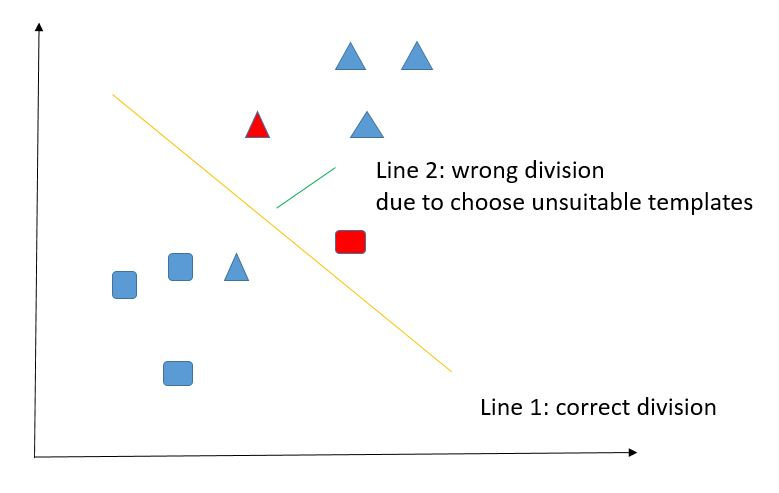
\includegraphics[width=0.8\linewidth]{SVM_better_than_uWave.JPG}
  \caption{SVM is better than uWave when we have similar gestures}
  \label{SVMuWave}
\end{figure} 
\subsection{Gesture control application}
Since now we have built the uWave on Android mobile phone. The application can input gesture library templates and recognize input gesture. We plan to build an application using gesture recognition. This phone application sends signals to blue tooth adapter connected to computer and let our application control the computer in the air! We plan to have following gestures:
\begin{enumerate}
  \item Control slide show: previous and next slide 
  \item Can write some English letters and numbers in air and recognize them. 
\end{enumerate}
We can show these cool work in course presentation.

\section{Conclusion}
TODO add this


%
% The following two commands are all you need in the
% initial runs of your .tex file to
% produce the bibliography for the citations in your paper.
\nocite{*}
\bibliographystyle{abbrv}
\bibliography{sigproc}  % sigproc.bib is the name of the Bibliography in this case

% That's all folks!
\end{document}
